%导言区
\documentclass[12pt]{ctexbook}  %article.book.report,letter   纯中文类可直接使用ctexart,ctexrep,ctexbook,并注释掉ctex宏包的引入

%\usepackage{ctex}		%处理中文
\usepackage{xltxtra}	%提供针对XeTex的改进并且加入XeTex的LOGO
\usepackage{texnames}
\usepackage{mflogo}
%\usepackage[backref]{hyperref}

\usepackage{url}	%Latex 中插入超链接 插入网址,第15页

\usepackage{amsmath} 
\usepackage{enumerate,mathdots} 
\usepackage{amssymb} %导入不编号公式,矩阵

\usepackage{cite}

%导言区:\usepackage{graphicx}
%语法:  \includegraphics[选项]{文件名}
%格式:  EPS,PDF,PNG,JPEG,BMP
\usepackage{graphicx}
\graphicspath{{figures/}} %图片全部存在当前目录的figures和pics目录中\graphicspath{{figures/},{pics/}}

\usepackage{verbatim}

\bibliographystyle{IEEEtran}

\usepackage{pythonhighlight}
%用\includegraphics[可选参数]{文件名}插入图像		参数选择有scale缩放因子,height图像高度,width图像宽度
%\includegraphics[scales=0.3]{文件名}
%\includegraphics[height=2cm]{文件名}
%\includegraphics[width=2cm]{文件名}
%\includegraphics[height=0.1\textheight]{文件名}	文本0.1倍的文本高度
%\includegraphics[width=0.1\textwidtn]{文件名}		文本0.1倍的文本宽度
%\includegraphics[angle=-45,width=0.1\textwidtn]{文件名}		旋转角度,文本0.1倍的文本宽度

%标题控制(caption,bicaption等宏包)
%并排与子图表(subcaption,subfig,floatrow等宏包)
%绕排(picinpar,wrapfig等宏包)


%\ctexset{
%	section ={
%		format+ = \zihao{-4} \heiti \raggedright,
%		name = {, }
%		number = \chinese{section}
%		beforeskip = 1.0ex plus 0.2ex minus .2ex,
%		afterskiip = 1.0ex plus	0.2ex minus .2ex,
%		aftername = \hspace{0pt}
%	},
%	subsection ={
%		format + = \zihao{-4} \heiti \raggedright,
%		name = {, }
%		number = \chinese{section}
%		beforeskip = 1.0ex plus 0.2ex minus .2ex,
%		afterskiip = 1.0ex plus	0.2ex minus .2ex,
%		aftername = \hspace{0pt}
%	},



\newcommand\degree{^\circ}	%定义degree命令

\title{\heiti 杂谈勾股定理}
\author{\kaishu 喜哥}
\date{\today}

%正文区
\begin{document}
	\maketitle
	Hello World!
	
	%常插入注释
	Let $f(x)$ be defined by the formula $f(x)=3x^2+x-1$.put another $$f(x)=3x^2+x-1$$which is a polynomial of degree 2
	
	勾股定理可以用现代语言表达如下:
	直角三角形斜边的平方等于两腰的平方和。
	可以用符号语言表达为:设直角三角形$ABC$,其中$\angle C=90\degree$,则有:
	\begin{equation}
		AB^2 = BC^2 + AC^2.
	\end{equation}

	%字体族设置(罗马字体,无衬线字体,打印机字体)两种方式
	\textrm{Roman Family} \textrm{Sans Serif Family}  \textrm{Typer Writer Family}
	
	{\rmfamily Roman Family} {\sffamily Sans Serif Family} {\ttfamily Typewriter Family}
	% 例子
	{\sffamily who you are? you find self on everyone around. take you as the same as others! }
	
	{\ttfamily Are you wiser }
	
	%字体系列设置(粗细,宽度)
	\textmd{Medium Series}  \textbf{Boldface Series}
	{\mdseries Medium Series}  {\bfseries Boldface Series}
	
	%字体形状(直立,斜体,伪斜体,小型大写)
	\textup{Upright Shape}  \textit{Italic Shape}
	\textsl{Slanted Shape}  \textsc{Small Caps Shape}
	%另一种表示方法
	{\upshape Upright Shape}  {\itshape Italic Shape}
	{\slshape Slanted Shape}  {\scshape Small Caps Shape}
	
	%中文字体 注意quad用法
	{\songti 宋体}  {\heiti 黑体}  \quad {\fangsong 仿宋}  \qquad {\kaishu 楷书}
	
	中文字体的\textbf{粗体}与\textit{斜体} 
	
	%字体大小,可在document设置字号配合使用
	\begin{table}[]
		\begin{tabular}{|l|ll|ll|l|l|l|}
			\hline
			\multicolumn{1}{|c|}{}       & \multicolumn{2}{l|}{zihao = 5} & \multicolumn{2}{l|}{zihao = -4} & 10pt & 11pt & 12pt \\ \cline{1-1}
			字体命令                         & 字号            & bp             & 字号            & bp              & pt   & pt   & pt   \\ \hline
			\textbackslash{}tiny         & 七号            & 5.5            & 小六            & 6.5             & 5    & 6    & 6    \\ \cline{1-1} \cline{6-8} 
			\textbackslash{}scriptsize   & 小六            & 6.5            & 六号            & 7.5             & 7    & 8    & 8    \\ \cline{1-1} \cline{6-8} 
			\textbackslash{}footnotesize & 六号            & 7.5            & 小五            & 9               & 8    & 9    & 10   \\ \cline{1-1} \cline{6-8} 
			\textbackslash{}small        & 小五            & 9              & 五号            & 10.5            & 9    & 10   & 11   \\ \cline{1-1} \cline{6-8} 
			\textbackslash{}normalsize   & 五号            & 10.5           & 小四            & 12              & 10   & 11   & 12   \\ \cline{1-1} \cline{6-8} 
			\textbackslash{}large        & 小四            & 12             & 小三            & 15              & 12   & 12   & 14   \\ \cline{1-1} \cline{6-8} 
			\textbackslash{}Large        & 小三            & 15             & 小二            & 18              & 14   & 14   & 17   \\ \cline{1-1} \cline{6-8} 
			\textbackslash{}LARGE        & 小二            & 18             & 二号            & 22              & 17   & 17   & 20   \\ \cline{1-1} \cline{6-8} 
			\textbackslash{}huge         & 二号            & 22             & 小一            & 24              & 20   & 20   & 25   \\ \cline{1-1} \cline{6-8} 
			\textbackslash{}Huge         & 一号            & 26             & 一号            & 26              & 25   & 25   & 25   \\ \hline
		\end{tabular}
	\end{table}
	
	\tableofcontents
	
	\chapter{绪论}
	\section{研究的目的和意义}
	
	近年来,随着逆向工程和三维重建技术的发展和应用,获取真实世界中物体的三维数据的方法越来越多的关注和研究,很多研究机构和商业公司都陆续推出了自己的三维重建系统。
	近年来,随着逆向工程和三维重建技术的发展和应用,\par 获取真实世界中物体的三维数据的方法越来越多的关注和研究。\\很多研究机构和商业公司都陆续推出了自己的三维重建系统。
	\section{国内外研究现状}
	\subsection{国外研究现状}
	\subsection{国内研究现状}
	\section{研究内容}
	\section{研究方法与技术路线}
	\subsection{研究内容}
	\subsection{技术路线}
	
	\chapter{实验与结果分析}
	\section{引言}
	\section{实验方法}
	\section{实验结果}
	\subsection{数据}
	\subsection{图表}
	\subsubsection{实验条件}
	\subsubsection{实验过程}
	\subsection{结果分析}
	\section{结论}
	\section{致谢}
	
	\chapter{LaTex特殊字符}
	\section{空白符号}
	%空行分段,多个空行等同与1个
	%自动缩进,绝对不能使用空格代替
	%英文中多个空格处理为1个空格,中文中的空格会被忽略
	%汉字与其他字符的间距会自动有XeLaTeX处理
	%禁止使用中文全角空格
	Are you wiser          than others? definitely no. in some ways, may it is ture. What can you achieve? a luxurious house? a brillilant car? an admirable career? who knows?
	近年来,随着逆向工程和三维重建技术的发展和应用,获取真实世界中物体的         三维数据的方法越来越多的关注和研究,很多研究机构和      商业公司都陆续推出了自己的三维重建系统。
	近年来,随着逆向工程和三维重建技术的发展和应用,获取真实世界中物体的in some ways三维数据的方法越来越多的关注和研究。很多研究机构和商业公司都陆续推出了自己的三维重建系统。
	
	% 1 em (当前字体中M的宽度)
	a\quad b
	
	% 2 em 
	a\qquad b
	
	% 约为1\6个em
	a\,b	a\thinspace b
	
	% 0.5个em
	a\enspace b
	
	%空格
	a\ b
	
	%硬空格
	a~b
	
	% 1pc=12pt=4.218cm
	a\kern 1pc b
	
	a\kern -1em b
	
	a\hskip 1em b
	
	%占位宽度
	a\hphantom{xyz}b
	
	%弹性长度
	a\hfill b
	\section{\LaTeX 控制符}
	\#
	
	\$
	
	\%
	
	\{ \}
	
	\~{}
	
	\_{}
	
	\^{}
	
	\textbackslash
	
	\&
	
	\section{排版符号}
	\S
	
	\P
	
	\dag
	
	\ddag
	
	\copyright
	
	\pounds
	
	\section{\TeX 标志符号}
	%基本符号
	\TeX{}
	
	\LaTeX{}
	
	\LaTeXe{}
	
	%xltxtra宏包提供
	\XeLaTeX{}
	
	%texnames宏包提供
	\AmSTeX{}
	
	\AmS-\LaTeX{}
	
	
	%mflogo宏包提供
	\METAFONT{}
	
	\MF{}
	
	\MP{}
	
	\section{引号}
	' `%1旁的 
	
	'' ``%两个
	
	``你好''
	\section{连字符}
	-
	
	--
	
	---
	\section{非英文字符}
	\oe
	
	\OE
	
	\ae
	
	\AE
	
	\aa
	
	\AA
	
	\o
	
	\O
	
	\l
	
	\L
	
	\ss
	
	\SS
	
	!`
	
	?`
	\section{重音符号(已O为例)}
	\`o
	
	\'o
	
	\^o
	
	\'`o
	
	\~o
	
	\=o
	
	\.o
	
	\u{o}
	
	\v{o}
	
	\H{o}
	
	\r{o}
	
	\t{o}
	
	\b{o}
	
	\c{o}
	
	\d{o}
	
	近年来,随着逆向工程和三维重\\建技术的发展和应用,获取真实
	
	世界中物体的三维数据的方法越来\\越多的关注和研究,很多研究机构和商业公司都陆\\续推出了自己的三维重建系统。
	近年来,随着逆向工程和三维重建技术的发展和应用,\par 获取真实世界中物体
	的三维数据的方法越来越多的关注和研究。\\很多研究机构和商业公司都\\陆续推出了自己的
	
	三维重建系统。
%	figure环境(table环境与之类似)
%	\begin{figure}[(允许位置)]
%		任意内容
%	\end{figure}
%	( 允许位置)参数(默认tbp)
%	h,此处(here)- 代码所在的上下文位置			
%	t,页顶(top)- 代码所在页面或之后页面的顶部
%	b,页底(bottom) - 代码所在页面或之后页面的底部
%	p,独立一页(page) - 浮动页面

% ctrl+t 快速注释		ctrl+u 去注释
	柏林大教堂:见图\ref{berlin}

	\begin{figure}[htbp]
		\centering
		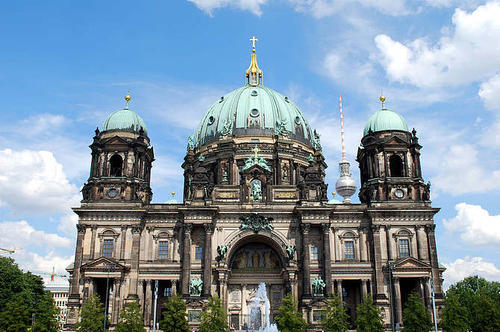
\includegraphics[scale=0.1]{0}
		\caption{柏林大教堂}
		\label{berlin}
	\end{figure}


	勃兰登堡门:见图\ref{wei}
	
	\begin{figure}[h]
		\centering
		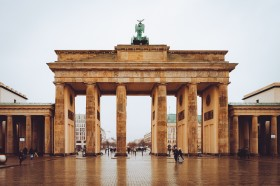
\includegraphics[scale=1.0]{1}
		\caption{勃兰登堡门}
		\label{wei}
	\end{figure}
	
	表格生成网站
	
	\url{https://tablesgenerator.com/latex_tables}
	
	
	\begin{table}[h]
		\centering
		\caption{字号表格}
		\label{chen}
		\begin{tabular}{|l|ll|ll|l|l|l|}
			\hline
			\multicolumn{1}{|c|}{}       & \multicolumn{2}{l|}{zihao = 5} & \multicolumn{2}{l|}{zihao = -4} & 10pt & 11pt & 12pt \\ \cline{1-1}
			字体命令                         & 字号            & bp             & 字号            & bp              & pt   & pt   & pt   \\ \hline
			\textbackslash{}tiny         & 七号            & 5.5            & 小六            & 6.5             & 5    & 6    & 6    \\ \cline{1-1} \cline{6-8} 
			\textbackslash{}scriptsize   & 小六            & 6.5            & 六号            & 7.5             & 7    & 8    & 8    \\ \cline{1-1} \cline{6-8} 
			\textbackslash{}footnotesize & 六号            & 7.5            & 小五            & 9               & 8    & 9    & 10   \\ \cline{1-1} \cline{6-8} 
			\textbackslash{}small        & 小五            & 9              & 五号            & 10.5            & 9    & 10   & 11   \\ \cline{1-1} \cline{6-8} 
			\textbackslash{}normalsize   & 五号            & 10.5           & 小四            & 12              & 10   & 11   & 12   \\ \cline{1-1} \cline{6-8} 
			\textbackslash{}large        & 小四            & 12             & 小三            & 15              & 12   & 12   & 14   \\ \cline{1-1} \cline{6-8} 
			\textbackslash{}Large        & 小三            & 15             & 小二            & 18              & 14   & 14   & 17   \\ \cline{1-1} \cline{6-8} 
			\textbackslash{}LARGE        & 小二            & 18             & 二号            & 22              & 17   & 17   & 20   \\ \cline{1-1} \cline{6-8} 
			\textbackslash{}huge         & 二号            & 22             & 小一            & 24              & 20   & 20   & 25   \\ \cline{1-1} \cline{6-8} 
			\textbackslash{}Huge         & 一号            & 26             & 一号            & 26              & 25   & 25   & 25   \\ \hline
		\end{tabular}
	\end{table}
	字号所对应表格\ref{chen}



	\chapter{数学公式初步}
	\LaTeX{}将排版内容分为文本模式和数学模式。文本模式用于普通文档排版,数学模式用于数学公式排版。
	\section{行内公式}
	\subsection{美元符号}
	交换率是$a+b=b+a$,如 $1+2=2+1=3$。
	\subsection{小括号}
	交换率是\(a+b=b+a\),如\(1+2=2+1=3\)。
	\subsection{math环境}
	交换律是\begin{math}
	1+2=2+1=3
	\end{math}
	\section{上下标}
	\subsection{上标}
	$3x^2 - x + 2 = 0$
	$3x^{3x^{20} - x + 2} - x + 2 = 0 $
	\subsection{下标}
	$a_0, a_1, a_2$
	
	$a_1, a_1, a_2, ..., a_{3x^{20} - x + 2}$
	\section{希腊字母}
	$\alpha$
	
	$\beta$
	
	$\gamma$
	
	$\epsilon$
	
	$\pi$
	
	$\omega$
	
	$\Gamma$
	
	$\Delta$
	
	$\Theta$
	
	$\Pi$
	
	$\Omega$

	$\alpha^3 + \beta^2 + \gamma = 0$
	\section{数学函数}
	$\log$
	
	$\sin$
	
	$\cos$
	
	$\arcsin$
	
	$\arccos$
	
	$\ln$
	
	$\sin^2 x + \cos^2 x = 1$
	
	$y = \arcsin x$
	
	$y = \sin^{-1} x$
	
	$y = \log_2 x$
	
	$y = \ln x$
	
	$\sqrt{2}$
	
	$\sqrt{x^2 + y^2}$
	
	$\sqrt{2 + \sqrt{2}}$
	
	$\sqrt[4]{x}$
	\section{分式}
	大约是原体积的$3/4$
	
	大约是原体积的$\frac{3}{4}$
	
	$\frac{x}{x^2 + x + 1}$
	
	$\frac{\sqrt{x-1}}{\sqrt{x+1}}$
	
	$\frac{1}{1 + \frac{1}{x}}$
	
	$\sqrt{\frac{x}{x^2 + x + 1}}$
	\section{行间公式}
	\subsection{美元符号}
	交换律是
	$$a+b=b+a$$
	如
	$$1+2=2+1=3$$
	\subsection{中括号}
	交换律是
	\[a+b=b+a\]
	如
	\[1+2=2+1=3\]
	\subsection{displaymath环境}
	交换律是
	\begin{displaymath}
		1+2=2+1=3
	\end{displaymath}
	\subsection{自动编号公式equation环境}
	交换律见式\ref{eq:commutative}
	\begin{equation}
		a+b=b+a		\label{eq:commutative}
	\end{equation}
	\subsection{不编号公式align*环境}
	交换律见式
	\begin{align*}
		a+b=b+a	%	\label{eq:commutative}
	\end{align*}

	公式的编号与交叉引用也是自动实现的,大家在排版中,要习惯于采用自动化的方式处理诸如图,表,公式的编号与交叉引用。再如公式\ref{eq:pol}
	\begin{equation}
		x^5 + 7x^3 + 4x = 0 \label{eq:pol}
	\end{equation}
	
	\chapter{公式矩阵}
	
	\[
	\begin{matrix}
		0 & 1\\1 & 0
	\end{matrix}
	\]
	
	\[
	\begin{pmatrix}
		0 & -i \\
		i & 0
	\end{pmatrix}
	\]
	
	\[
	\begin{bmatrix}
		0 & -1 \\
		1 & 0
	\end{bmatrix}
	\]
	
	\[
	\begin{Bmatrix}
		1 & 0 \\ 0 & -1
	\end{Bmatrix}
	\]
	
	\[
	\begin{vmatrix}
		a & b \\
		c & d
	\end{vmatrix}\]

	\[
	\begin{Vmatrix}
		a & b \\ c & d
	\end{Vmatrix}
	\]
	%可以使用上下标
	\[
	A = \begin{pmatrix}
		a_{11}^2 & a_{12}^2 & a_{13}^2 \\
		0 & a_{22} & a_{23} \\
		0 & 0 & a_{33}
	\end{pmatrix}
	\]
	%常用省略号:\dots,\vdots,\ddots,\adots
	\[
	A = \begin{bmatrix}
		a_{11} & \dots & a_{1n} \\
		\vdots & \ddots & \vdots \\
		0 & \cdots & a_{nn}
	\end{bmatrix}_{n \times n}
	\]
	%分块矩阵(矩阵嵌套)
	\[
	\begin{pmatrix}
	\begin{matrix}
		1&0\\0&1
	\end{matrix}
	& \text{\Large 0} \\
	\text{\Large 0} & \begin{matrix}
		1&0\\0&-1
	\end{matrix}
	\end{pmatrix}
	\]
	%三角矩阵
	\[
	\begin{pmatrix}
		a_{11} & a_{12} & \cdots & a_{1n} \\
		& a_{22} & \cdots & a_{2n} \\
		&        & \ddots & \vdots \\
		\multicolumn{2}{c}{\raisebox{1.3ex}[0pt]{\Huge 0}}
		&        &a_{nn}
	\end{pmatrix}
	\]
	%行内小矩阵(smallmatrix)环境
	复数 $Z = (x,y)$ 也可用矩阵
	\begin{math}
		\left(
		\begin{smallmatrix}
			x & -y \\ y & x
		\end{smallmatrix}
		\right)
	\end{math}来表示
	%array 环境(类似于表格环境tabular)
	\[
	\begin{array}{r|r}
		\frac12 & 0 \\
		\hline
		0 & -\frac abc \\
	\end{array}
	\]
	%用array环境构造复杂矩阵
	
%\cdots是横向的省略号
%\vdots是竖向的省略号
%\ddots是对角线方向的省略号
%\ldots 是跟文本底线对齐的省略号
	
	\[
	%@{内容}-添加任意内容,不占表项计数
	%此处添加一个负值空白,表示向左移-5pt的距离
	\begin{array}{c@{\hspace{-5pt}}l}
		\left(
		\begin{array}{ccc|ccc}
		a & \cdots & a & b & \cdots & b\\
		& \ddots & \vdots & \vdots &  \ddots  \\
		&        & a & b \\  \hline
		&        &   & c & \cdots & c\\
		&        &   & \vdots & & \vdots\\
		\multicolumn{3}{c |}{\raisebox{2ex}[0pt]{\Huge 0}}
		& c & \cdots & c
		\end{array}
		\right)
		&
		\begin{array}{l}
		%\left.仅表示与\right配对,什么都不输出
		\left.\rule{0mm}{7mm}\right\}p\\
		\\
		\left.\rule{0mm}{7mm}\right\}q
		\end{array}
		\\[5pt]
		\begin{array}{cc}
			\underbrace{\rule{17mm}{0mm}}_m &
			\underbrace{\rule{17mm}{0mm}}_m 
		\end{array}
		&
	\end{array}
	\]
	\chapter{数学公式的多行公式}
	%带编号
	\begin{gather}
		a + b = b + a \\
		ab  ba
	\end{gather}
	%不带编号
	\begin{gather*}
		3 + 5 = 5 + 3 =8 \\
		3 \times 5 = 5 \times 3
	\end{gather*}
	%在\\前使用\notag阻止编号
	\begin{gather}
		3^2 + 4^2 = 5^2 \notag \\
		5^2 + 12^2 = 13^2 \notag \\
		a^2 + b^2 = c^2
	\end{gather}
	%align和align*环境(用&进行对齐)
	%带编号
	\begin{align}
		x &= t + \cos t + 1 \\
		y &= 2\sin t
	\end{align}
	%不带编号
	\begin{align*}
		x &= t & x &= \cos t & x &= t \\
		y &= 2t & y &= \sin(t+1) & y &= \sin t
	\end{align*}
	%split环境(对采用align环境的方式,编号在中间)
	\begin{equation}
	\begin{split}
		\cos 2x &= \cos^2 x - \sin^2 x \\
		&= 2\cos^2 x - 1
	\end{split}
	\end{equation}
	%cases 环境
	%每行公式中使用&分隔为两部分,通常表示值和后面的条件
	\begin{equation}
		D(x) = \begin{cases}
			1, & \text{如果 } x \in \mathbb{Q}; \\
			0, & \text{如果 } x \in \mathbb{R}\setminus\mathbb{Q}.
		\end{cases}
	\end{equation}

$$\textbf{0}= \begin{aligned}
	\begin{bmatrix}
		0 \\0  \\ \vdots \\ 0
	\end{bmatrix}
\end{aligned}$$ 


$$\textgreater$$


	%一次管理,一次使用
	%参考文献格式:
	%\begin{thebibliography}{样本编号}
	%	\bibitem[记号]{引用标志}文献条目1
	%	\bibitem[记号]{引用标志}文献条目1
	%	...
	%\end{thebibliography}
	%其中文献条目包括:作者,题目,出版社,年代,版本,页码等
	%引用时候要采用:\cite{引用标志1,引用标志2,...}
	\chapter{参考文献排版}
	引用一篇文章\cite{artcle1} 引用一本书\cite{book1}等等	\texttt{http://www.zotero.org}
	\begin{thebibliography}{99}
		\bibitem{artcle1}陈立辉,苏伟,蔡川,陈晓云,\emph{基于LaTex的Web数学公式提取方法研究}[J].计算机科学.2014(06)
		
		\bibitem{book1}William H. Press,Saul A. Teukolsky, William T. Vetterling,Brian P. Flannery,
		\emph{Numerical Recipes 3rd Edition: The Art of Scientific Computing} Cambridge University Press, New York,2007.
		
		\bibitem{latexGuide} Kopka Helmut, W. Daly Patrick,
		\emph{Guide to \LaTeX}, $4^{th}$ Edition.
		Available at \texttt{http://www.amazon.com}.
		
		\bibitem{latexMath} Graetzer Georgr, \emph{Math Into \LaTeX},
		Birkhuser Boston; 3 edition (June 22, 2000).
	\end{thebibliography}
	这是一个来自于知网的文献:\cite{dosovitskiy2020image}
	
	%\bibliographystyle{IEEEtran}
	\bibliography{cnki.bib}
	
	\begin{comment}
		perceptilabs:pip install perceptilabs
		kite(代码工具):https:www.kite.com/
		HDF5(.h5数据查看器):https://portal.hdfgroup.org/display/support/HDFView+3.1.2#files
		wget(压缩包下载与解压命令):https://eternallybored.org/misc/wget/
		
		paddlepaddle(飞桨官网):https://www.paddlepaddle.org.cn/	
		pytorch:https://pytorch.org/get-started/locally/
		tensorflow:https://tensorflow.google.cn/versions/r2.4/api_docs?hl=en
		(在PYPI和Python Extension Packages上下载安装,记得加上GPU):  
		https://mirrors.tuna.tsinghua.edu.cn/pypi/web/simple/tensorflow/
		https://www.tensorflow.org/install/source_windows
		
		Visual Studio:https://visualstudio.microsoft.com/zh-hans/downloads/
		Pytorch官网:http://pytorch.org
		CUDA的下载地址:https://developer.nvidia.com/cuda-toolkit-archive
		CUDNN的安装https://developer.nvidia.com/rdp/cudnn-archive
		
		数据库:https://hyper.ai/datasets
		MADS数据集:数据集包含5种分类,共计5万3千帧
		LSP数据集:体育姿态数据集,2000个姿态注释
		FLIC数据集:电影帧标记人物数据集
		
		kaggle网上的数据集:https://www.kaggle.com   
		MPLL数据集:http://human-pose.mpi-inf.mpg.de/#download
		COCO数据集:https://cocodataset.org/#download
		HumanEva Dataset:http://humaneva.is.tue.mpg.de/(walking,jogging,gesturing,etc)
		CIFAR-100 Dataset: 是用于机器视觉领域的图像分类数据集
		
		
		论文集https://arxiv.org/
		顶级期刊CVPR,ECCV,ICCV:https://openaccess.thecvf.com/menu
		
		python 第三方安装包:Unofficial Windows Binaries for Python Extension Packages:https://www.lfd.uci.edu/~gohlke/pythonlibs/#scikits.ann    
							PYPI:https://pypi.org/
		python函数使用源码:https://codingdict.com/sources/py/all
		python官方网站:https://docs.python.org/zh-cn/3.7/
		
		Latex表格生成:https://tablesgenerator.com/latex_tables
		Latex公式生成:https://latexeditor.lagrida.com/
		Latex模板:https://www.ctan.org/tex-archive/info/lshort/
		
		stanfordcs229:http://cs229.stanford.edu/syllabus-spring2021.html
		
		PCL:https://robotica.unileon.es/index.php?title=Home
		数值分析软件:https://www.gnu.org/software/octave/
		
		pillow:https://pillow.readthedocs.io/en/stable/index.html#
		scipy:http://scipy.github.io/devdocs/tutorial/index.html
		opencv:https://docs.opencv.org/4.2.0/dc/d3a/classcv_1_1viz_1_1Camera.html
		
		各种系统的iso文件下载: https://next.itellyou.cn/Original/
	\end{comment}
		

	
			
\end{document}
